\documentclass[aspectratio=169]{beamer}
\usetheme{Madrid}
\usepackage[utf8]{inputenc}
\usepackage[T1]{fontenc}
\usepackage{tikz}
\usepackage{amssymb}
\usepackage{graphicx}
\setbeamertemplate{navigation symbols}{}
\setbeamercolor{title}{fg=white,bg=blue!70!cyan}
\setbeamercolor{frametitle}{fg=white,bg=blue!70!cyan}
\setbeamercolor{block title}{bg=blue!70!cyan!20,fg=black}
\setbeamercolor{block body}{bg=blue!70!cyan!8,fg=black}
\setbeamercolor{item}{fg=blue!70!cyan}
\setbeamercolor{itemize item}{fg=blue!70!cyan}
\setbeamertemplate{itemize item}[triangle]

\title{Tier 3 — Signals \& Decisions}
\subtitle{Real IF-based decisions on real data the mission gives you}
\author{ByteForge --- Grade 9 --- The Deep Diver}
\date{}

\begin{document}

\begin{frame}
    \titlepage
\end{frame}

\begin{frame}{Today's Missions}
    \Large
    \begin{itemize}
        \item Beacon Run
        \item Three-Way Beacon
        \item Alternating Signal Beacons
    \end{itemize}
\end{frame}

\begin{frame}{IF --- a real decision, not a fixed pattern}
    \large
    \begin{itemize}
        \item Beacon colours (G, R, G) are real DATA your code reads and reacts to
        \item G turns left, R turns right --- your FIRST mission requiring a genuine decision
    \end{itemize}
\end{frame}


\begin{frame}{if / elif / else --- three-way decisions}
    \large
    \begin{itemize}
        \item Three colours need a THREE-way decision, not just if/else
        \item Only the FIRST matching branch runs --- checked top to bottom
        \item "Do nothing" (fly straight) is a real, valid branch too
    \end{itemize}
\end{frame}


\begin{frame}{MOD/\% uses a number's POSITION, not just its value}
    \large
    \begin{itemize}
        \item \texttt{enumerate()} gives you BOTH the index and the value together
        \item \texttt{i \% 2} --- remainder 0 means even position, remainder 1 means odd
        \item This is exactly how every "every other item" pattern in real code works
    \end{itemize}
\end{frame}

\begin{frame}{Real-World Examples}
    \large
    \begin{itemize}
        \item A pedestrian crossing button genuinely reads a real signal (has it been pressed?) and reacts with a real decision (change the light eventually).
    \end{itemize}
\end{frame}


\begin{frame}{Image}
    \begin{center}
    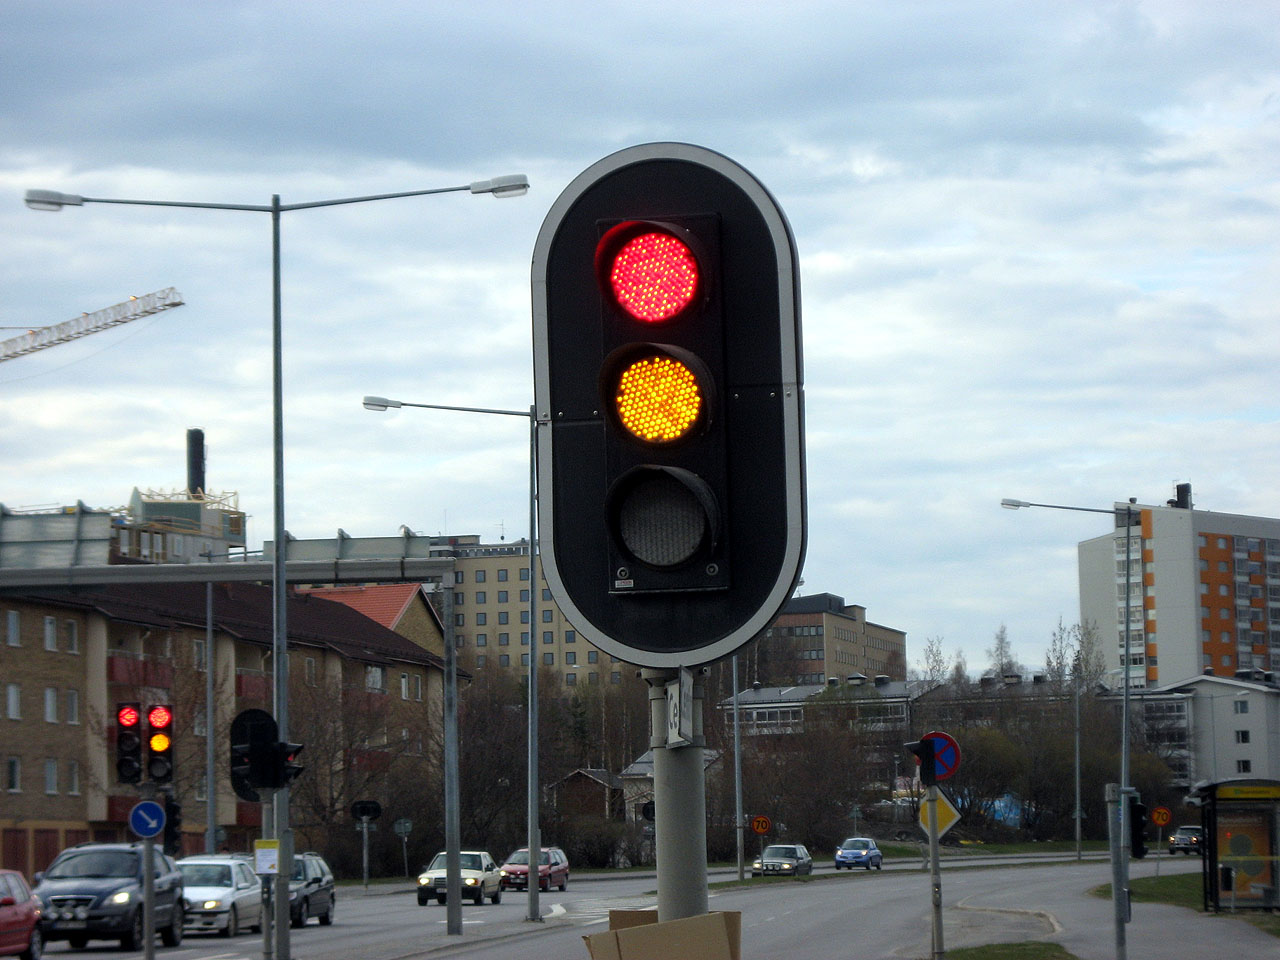
\includegraphics[width=0.5\textwidth]{images/traffic.jpg}

    \large A real traffic light is a real three-way decision --- red, amber, or green, exactly one branch active at a time.

    \small LED traffic lights, public domain (PD-self), via Wikimedia Commons
    \end{center}
\end{frame}

\begin{frame}{Let Them Discover}
    \large
    Watch a real traffic light for a few minutes. What are the THREE states, and does it ever skip straight from red to green with no amber?
\end{frame}

\begin{frame}{Your Turn}
    \Large
    Open the mission map, find \textbf{Tier 3 — Signals \& Decisions}, and fly it for real ---
    everything you just saw, you now do yourself.
\end{frame}

\end{document}
